\documentclass{article}
    \usepackage{amssymb}
    \usepackage[utf8]{inputenc}
    \usepackage[russian]{babel}
    \usepackage[left=2cm,right=2cm,
        top=2cm,bottom=2cm,bindingoffset=0cm]{geometry}
    \usepackage{hyperref}
    \hypersetup{
        colorlinks=true,
        linkcolor=blue,
        filecolor=magenta,      
        urlcolor=cyan,
    }
  \usepackage{graphicx}
  \graphicspath{{pictures/}}
  \DeclareGraphicsExtensions{.pdf,.png,.jpg}
\usepackage{subcaption}
%\captionsetup{compatibility=false}

\begin{document}
\begin{center}{\hugeОтчет по курсовой работе за неделю\\}\end{center}
Дата: 26.11.2020\\
Научные руководители: Герасимов С.В., Мещеряков А.В.\\
Студент: Немешаева Алиса\\
Курс: 4\\

\renewcommand{\labelitemi}{$\blacksquare$}
\renewcommand\labelitemii{$\square$}
\begin{enumerate}
    \item На этой неделе продолжилась работа над статьёй по каталогам дететированных скоплений. 
        Изменена структура, исправлены все основные разделы. Добавлено подробное описание каталогов 
        и данных, подробное описание практической части.\\
    \item \hyperlink{https://www.overleaf.com/read/zcgvtyscsyhv}{Статья.}\\
    \item Для классификации опробованы другие варианты моделей: Multilayer Perceptron, Random 
        Forest.\\ 
    
        \begin{figure}[h]

            \begin{subfigure}{0.5\textwidth}
                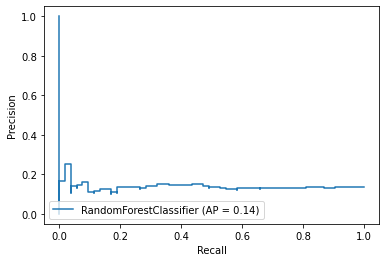
\includegraphics[width=0.7\linewidth]{pres_recall} 
                \caption{Кривая presicion-recall для Random Forest}
            \end{subfigure}
            \begin{subfigure}{0.5\textwidth}
                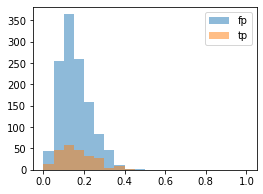
\includegraphics[width=0.7\linewidth]{hist}
                \caption{Распределение предсказаний с вероятностью по tp и fp объектам из 
                    детектированного каталога}
            \end{subfigure}

        \caption{Результаты классификации Random Forest}
        \end{figure}
    \item Построены маски для объектов: Shapley, Abell 399, Coma Cluster, Leo Cluster.\\
        \begin{figure}[h]
                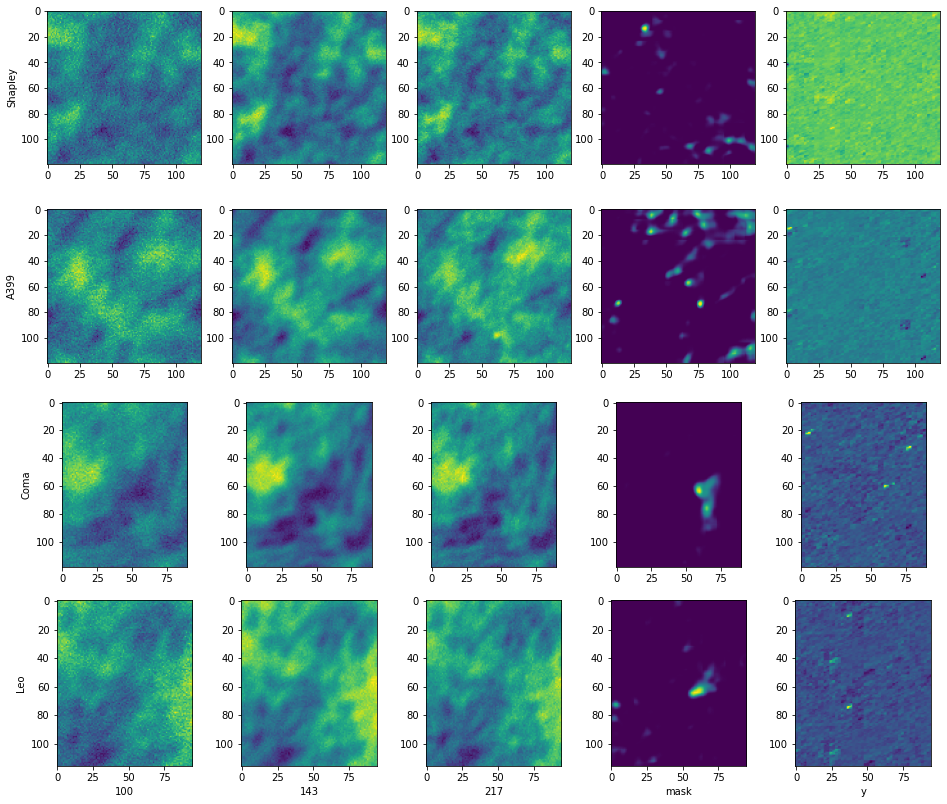
\includegraphics[width=0.7\linewidth]{4clusters} 
                \caption{Первые три канала карт Planck, маска prediction index и карта y-параметра
                    для упомянутых объектов}
        \end{figure}

\end{enumerate}

Отчет согласован с научным руководителем.\\
Общее количество строк кода за эту неделю: 201\\
\hyperlink{https://github.com/rt2122/data-segmentation-2}{Репозиторий}\\ 
\end{document}
